\documentclass[a4paper, 12pt]{article}
\usepackage{geometry}
\usepackage[russian]{babel}
\usepackage[T2A]{fontenc}
\usepackage{chngcntr}
\usepackage{graphicx}
\usepackage{verbatim}

\begin{document}


\begin{titlepage}

\begin{center}
{\textsc{\textbf{Правительство Российской Федерации}}}\\
\vspace{0.5cm}
\hrule
\vspace{0.5cm}
{\textsc{Федеральное государственное автономное образовательное учреждение\\высшего образования <<Национальный исследовательский университет\\<<Высшая школа экономики>>}}\\
\vspace{1cm}
Кафедра <<Компьютерная безопасность>>
\end{center}

\vspace{\fill}
% Поменять номер лабы
\begin{center}
{\Large{\textbf{ОТЧЕТ \\ К ЛАБОРАТОРНОЙ РАБОТЕ №13}}} \\
\vspace{1em}
{\textbf{по дисциплине}} \\
\vspace{1em}
{\large{\textbf{<<Языки программирования>>}}}
\end{center}

\vspace{\fill}


\begin{flushright}
  \begin{minipage}[center]{15cm}

    \begin{minipage}[left]{5cm}
      {Работу выполнил\\студент группы СКБ-222}
    \end{minipage}
    \begin{minipage}[center]{5cm}
      \vspace{1.25cm}
      \hrulefill\\[-1cm]
      \begin{center}{подпись, дата}\end{center}
    \end{minipage}
    \begin{minipage}[right]{4cm}
      \vspace{0.4cm}
      \begin{flushright}{А.С. Вагин}\end{flushright}
    \end{minipage}
    \\
    \\
    \\
    \begin{minipage}[left]{5cm}
      {Работу проверил}
    \end{minipage}
    \begin{minipage}[center]{5cm}
      \vspace{1.25cm}
      \hrulefill\\[-1cm]
      \begin{center}{подпись, дата}\end{center}
    \end{minipage}
    \begin{minipage}[right]{4cm}
      \begin{flushright}{С.А. Булгаков}\end{flushright}
    \end{minipage}
  \end{minipage}
\end{flushright}

\vspace{\fill}

\begin{center}
Москва~2023
\end{center}
\end{titlepage}
\setcounter{page}{2}
\setcounter{secnumdepth}{5}
\setcounter{tocdepth}{5}

% Содержание
\tableofcontents
\cleardoublepage

\setcounter{section}{1}
\counterwithout{subsection}{section}
\graphicspath{ {./images/} }

% Постановка задачи
\cleardoublepage
\section*{Постановка задачи}\addcontentsline{toc}{section}{Постановка задачи}
Реализовать алгоритм обработки данных (на свое усмотрение), а также его 
параллельную версию с использованием возможностей `std::thread`.
\\\\
\textbf{Основы профилирования - измерение быстродействия} \\
Получить эмпирическую зависимость изменения быстродействия от объема 
данных при фиксированном числе параллельных потоков используя возможности 
`std::chrono`.
\\\\
\textbf{Закон Амдала} \\
Построить теоретическую оценку увеличения быстродействия при фиксированном 
объеме данных и различном числе параллельных потоков.
Получить эмпирическое подтверждение построенной теоретической оценки спользуя 
возможности `std::chrono`.

\cleardoublepage



\section*{Основная часть}\addcontentsline{toc}{section}{Основная часть}

\subsection{Класс Matrix}
Для данной лабораторной работы был разработан класс Matrix, позволяющий хранить
любой тип данных в матрице. Реализация всех методов взята из лабораторной работы
№10.

\subsection{Описание функций}
\subsubsection{Функция \textit{determinant}}
Данная функция выполняет расчет определителя у матриц размера 2х2 и 1х1.

\subsubsection{Функция \textit{matrix\_below}}
Данная функция принимает на вход объект типа \textit{Matrix}, и возвращает
массив из объектов того же типа, однако возвращаемые матрицы на 1 размер меньше.
(Матрица 3х3 превращается в массив из 3 матриц 2х2) \\
Функция реализована для возможности линейного расчета определителя при помощи
миноров.

\subsubsection{Функция \textit{calculateDeterminant}}
Данная функция представляет собой сам алгоритм расчета определителя. На вход получает
объект типа \textit{Matrix} и объект типа long, переданный по ссылке.
Последний объект нужен для записи результата работы функции при использовании
потоков. Алгоритм преобразовывает матрицы при помощи функции \textit{matrix\_below}
до размера 2х2, после чего подсчитывает сумму определителей всех получившихся матриц при
помощи \textit{determinant}. Записывает результат в объект типа long, возвращает
сумму в виде локального объекта long.

\subsubsection{Функции \textit{randomMatrix} и \textit{randomSizeMatrix}}
Функции реализованы для создания матриц со случайными значениями. Отличие между ними
заключается в возможности изначально задать размер матрицы в функции \textit{randomMatrix},
когда в функции \textit{randomSizeMatrix} размер выбирается случайно. 

\subsubsection{Функция \textit{linear\_algorithm}}
Данная функция использует \textit{calculateDeterminant} последовательно,
не используя возможности многопоточности. Используется для сравнения с 
параллельным алгоритмом.

\subsubsection{Функция \textit{parallel\_algorithm}}
Функция использует алгоритм расчета определителей с возможностями многопоточности.

\subsubsection{Функция \textit{checkAlgorithm}}
Получает на вход объект типа \textit{Matrix}. Используя \textit{chrono}, 
замеряет время выполнения \textit{linear\_algorithm} и \textit{parallel\_algorithm}.
Выводит все результаты в поток вывода.

\subsubsection{Функция \textit{main}}
Входная точка программы. Используется для запуска и демонстрирует возможности реализованного алгоритма.

\cleardoublepage

\subsection{Измерение быстродействия}
Сравнение алгоритма с фиксированным количеством потоков (2) и последовательного
алгоритма с изменяющимся объемом данных. \\
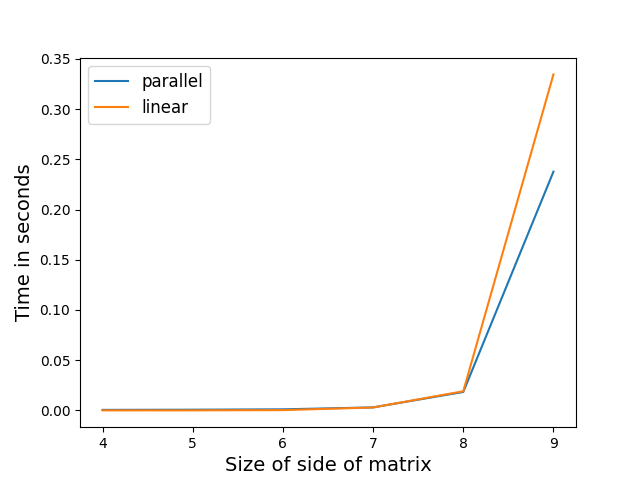
\includegraphics{plot1.png} 

\cleardoublepage

\subsection{Проверка закона Амдала}
Алгоритм с изменяющимся количеством потоков и статичным объемом данных (матрица 7х7). \\
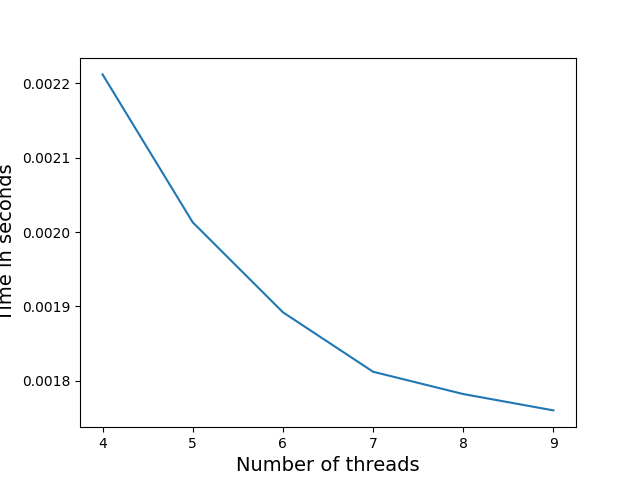
\includegraphics{plot2.png} 

\cleardoublepage


\section*{Приложение A}\addcontentsline{toc}{section}{Приложение А}
\renewcommand\thesection{\Alph{section}}
\renewcommand\thesubsection{\thesection.\arabic{subsection}}
\setcounter{subsection}{0}

\subsection{UML-диаграмма \textit{Matrix}}
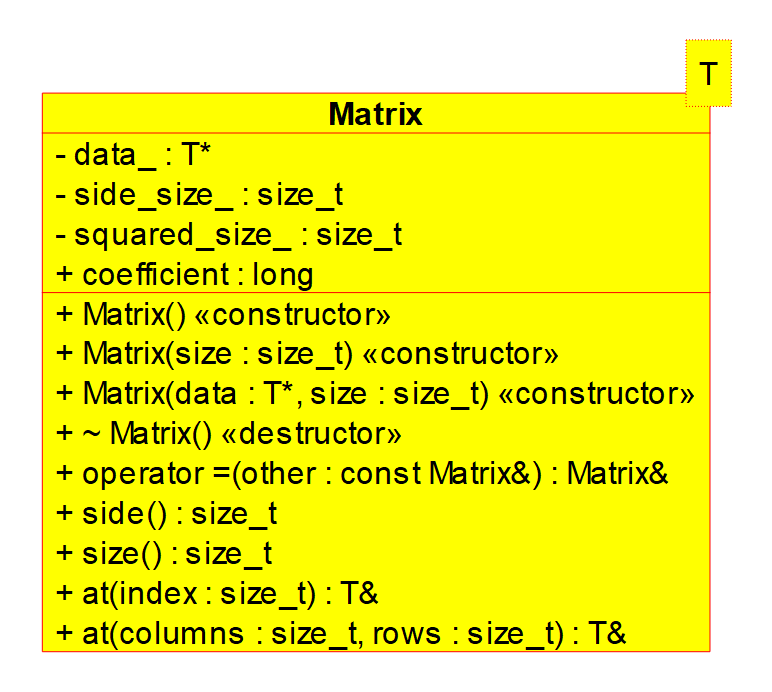
\includegraphics[width=\columnwidth]{uml.png}


\cleardoublepage

\setcounter{subsection}{0}
\section*{Приложение B}\addcontentsline{toc}{section}{Приложение B}
\renewcommand\thesection{\Alph{section}}
\renewcommand\thesubsection{B.1}

\subsection{Код файла \textit{Matrix.hpp}}

\fontsize{9}{9}\selectfont
% Код сюда
\begin{verbatim}
#ifndef MATRIX_TEMPLATE
#define MATRIX_TEMPLATE 09022023L

#include <iostream>

template <typename T>
class Matrix {
    private:
        T* data_;
        size_t side_size_;
        size_t squared_size_;
    
    public:
        long coefficient = 1;
        Matrix(): side_size_(0), data_(NULL), squared_size_(0) {}
        Matrix(size_t size): side_size_(size), data_(new T[size * size]), squared_size_(size * size) {}
        Matrix(T* data, size_t size): side_size_(size), squared_size_(size * size) {
            data_ = new T[squared_size_];
            for (size_t i = 0; i < squared_size_; ++i) {
                data_[i] = data[i];
            }
        }
        ~Matrix() {
            delete[] data_;
        }

        Matrix& operator=(const Matrix& other) {
            if (this == &other) return *this;

            if (data_) delete[] data_;

            this->side_size_ = other.side_size_;
            this->squared_size_ = other.squared_size_;
            this->data_ = new T[this->squared_size_];
            this->coefficient = other.coefficient;

            for (size_t i = 0; i < this->squared_size_; ++i) {
                data_[i] = other.data_[i];
            }

            return *this;
        } 

        size_t side() const {
            return side_size_;
        }

        size_t size() const {
            return squared_size_;
        }

        T& at(size_t index) {
            return data_[index];
        }
        const T& at(size_t index) const {
            return data_[index];
        }
        T& at(size_t columns, size_t rows) {
            return data_[side_size_ * columns + rows];
        }
        const T& at(size_t columns, size_t rows) const {
            return data_[side_size_ * columns + rows];
        }

        template <class U>
        friend std::ostream& operator<< (std::ostream& out, const Matrix<U>& matrix);
        
};

template <class U>
std::ostream& operator<<(std::ostream& out, const Matrix<U>& matrix) {   
    size_t i, u;
    for (i = 0; i < matrix.side_size_; ++i) {
        for (u = 0; u < matrix.side_size_; ++u) {
            out << matrix.at(i, u) << '\t';
        }
        out << std::endl;
    }
    return out; 
}

#endif /* MATRIX_TEMPLATE */
\end{verbatim}

\renewcommand\thesubsection{B.1}

\subsection{Код файла \textit{main.cpp}}

\fontsize{9}{9}\selectfont
\begin{verbatim}
#include <iostream>
#include <thread>
#include <chrono>
#include "Matrix.hpp"
#include <iomanip>

template <typename T>
long determinant(const Matrix<T>& matrix) {
    if (matrix.side() == 1) return matrix.coefficient * matrix.at(0);
    return matrix.coefficient * (matrix.at(0) * matrix.at(2) - matrix.at(1) * matrix.at(3));
}

template <typename T>
Matrix<T>* matrix_below(const Matrix<T>& base) {
    size_t i, u, counter;
    Matrix<T>* to_return = new Matrix<T>[base.side()]();
    Matrix<T> current (base.side() - 1);
    for (i = 0; i < base.side(); ++i) {
        current.coefficient = base.coefficient * base.at(i);
        if (i % 2 != 0) current.coefficient *= (-1);
        counter = 0;
        for (u = 0; u < base.size(); ++u) {
            if ((u + 1 > base.side()) && (u % base.side() != i)) {
                current.at(counter) = base.at(u);
                ++counter;
            }
        }
        to_return[i] = current;
    }
    return to_return;
}

template <typename T>
long calculateDeterminant(const Matrix<T>& base, long& to_write) {
    size_t i, u, current_side_size, current_size = 1;
    long to_return = 0;
    Matrix<T>* returned_matrixes = NULL, *current_matrixes = NULL;
    Matrix<T>* matrixes = new Matrix<T>[current_size]();
    matrixes[0] = base;
    while (matrixes[0].size() > 0) {
        if (matrixes[0].size() <= 2) {
            for (i = 0; i < current_size; ++i) {
                to_return += determinant(matrixes[i]);
            }
            break;
        }

        if (current_matrixes) delete[] current_matrixes;
        current_side_size = matrixes[0].side();
        current_matrixes = new Matrix<T>[current_size * current_side_size]();
        for (i = 0; i < current_size; ++i) {
            returned_matrixes = matrix_below(matrixes[i]);
            for (u = 0; u < current_side_size; ++u) {
                current_matrixes[i * current_side_size + u] = returned_matrixes[u];
            }
        }
        current_size *= current_side_size;
        delete[] matrixes;
        matrixes = new Matrix<T>[current_size]();
        for (i = 0; i < current_size; ++i) {
            matrixes[i] = current_matrixes[i];
        }
    }

    to_write += to_return;

    return to_return;
}

template <typename T>
long linear_algorithm(const Matrix<T>& matrix) {
    long determinant = 0;
    calculateDeterminant<long>(matrix, std::ref(determinant));
    return determinant;
}

template <typename T>
long parallel_algorithm(const Matrix<T>& matrix) {
    long determinant = 0;
    Matrix<T>* matrixes = matrix_below(matrix);
    for (size_t i = 0; i < matrix.side(); ++i) {
        std::thread current (calculateDeterminant<T>, matrixes[i], std::ref(determinant));
        current.join();
    }
    return determinant;
}

Matrix<long> defaultMatrix() {
    int size_of_matrix = 4;
    long* numbers = new long[16]{11, 19, 3, 12, 2, 86, 43, 16, 64, 3, 7, 4, 6, 4, 13, 6};
    Matrix<long> matrix (numbers, size_of_matrix);
    return matrix;
}

Matrix<long> randomMatrix(size_t size_of_matrix) {
    srand(time(0));
    long* numbers = new long[size_of_matrix * size_of_matrix];
    for (size_t i = 0; i < size_of_matrix * size_of_matrix; ++i) {
        numbers[i] = rand() % 40;
    } 
    Matrix<long> matrix (numbers, size_of_matrix);
    return matrix;
}

Matrix<long> randomSizeMatrix() {
    srand(time(0));
    size_t size_of_matrix = 4 + rand() % 6;
    return randomMatrix(size_of_matrix);
}

template <typename T>
void checkAlgorithm(const Matrix<T>& matrix) {
    long determinant1 = 0;
    long determinant2 = 0;

    std::cout << "Matrix: " << std::endl << matrix << std::endl << std::endl;

    auto start1 = std::chrono::steady_clock::now();
    determinant1 = linear_algorithm<long>(matrix);
    auto end1 = std::chrono::steady_clock::now();
    std::chrono::duration<double> elapsed_linear = end1 - start1;

    auto start2 = std::chrono::steady_clock::now();
    determinant2 = parallel_algorithm<long>(matrix);
    auto end2 = std::chrono::steady_clock::now();
    std::chrono::duration<double> elapsed_parallel = end2 - start2;

    std::cout << "Linear algorithm's determinant: " << determinant1 << std::endl;
    std::cout << "Linear algorithm's time (s): " << elapsed_linear.count() << std::endl;
    std::cout << "Parallel algorithm's determinant: " << determinant2 << std::endl;
    std::cout << "Parallel algorithm's time (s): " << elapsed_parallel.count() << std::endl << std::endl;
    // std::cout << std::fixed << std::setprecision(10);
    // std::cout << elapsed_linear.count() << std::endl;
}

int main() {
    Matrix<long> matrix = defaultMatrix();    
    checkAlgorithm(matrix);
    checkAlgorithm(randomSizeMatrix());
    return 0;
}
\end{verbatim}

\end{document}